% Template for a Computer Science Tripos Part II project dissertation
\documentclass[12pt,a4paper,twoside,openright]{report}
\usepackage[pdfborder={0 0 0}]{hyperref}    % turns references into hyperlinks
\usepackage[margin=25mm]{geometry}  % adjusts page layout
\usepackage{graphicx}  % allows inclusion of PDF, PNG and JPG images
\usepackage{verbatim}
\usepackage{pdfpages} % allows inclusion of non tex project proposal
\usepackage{docmute}   % only needed to allow inclusion of proposal.tex

\raggedbottom                           % try to avoid widows and orphans
\sloppy
\clubpenalty1000%
\widowpenalty1000%

\renewcommand{\baselinestretch}{1.1}    % adjust line spacing to make
                                        % more readable

\begin{document}

\bibliographystyle{plain}


%%%%%%%%%%%%%%%%%%%%%%%%%%%%%%%%%%%%%%%%%%%%%%%%%%%%%%%%%%%%%%%%%%%%%%%%
% Title


\pagestyle{empty}

\rightline{\LARGE \textbf{Oliver Black}}

\vspace*{60mm}
\begin{center}
\Huge
\textbf{Software IPv6 Router in Rust} \\[5mm]
Computer Science Tripos -- Part II \\[5mm]
Selwyn College \\[5mm]
\today  % today's date
\end{center}

\newpage
\section*{Declaration of Originality}

I, Oliver Black of Selwyn College, being a candidate for Part II of 
the Computer Science Tripos, hereby declare
that this dissertation and the work described in it are my own work,
unaided except as may be specified below, and that the dissertation
does not contain material that has already been used to any substantial
extent for a comparable purpose.

\bigskip
\leftline{Signed Oliver Black}

\medskip
\leftline{Date \today}

%%%%%%%%%%%%%%%%%%%%%%%%%%%%%%%%%%%%%%%%%%%%%%%%%%%%%%%%%%%%%%%%%%%%%%%%%%%%%%
% Proforma, table of contents and list of figures

\pagestyle{plain}

\chapter*{Proforma}

{\large
\begin{tabular}{ll}
Name:               & \bf Oliver Black                      \\
College:            & \bf Selwyn College                     \\
Project Title:      & \bf Software IPv6 Router in Rust \\
Examination:        & \bf Computer Science Tripos -- Part II, July 2001  \\
Word Count:         & \bf "FIX ME\& footnote" \footnotemark[1]
                       \\
Project Originator: & Oliver Black \& Dr Richard Watts      \\
Supervisor:         & Andrew Moore                   \\ 
\end{tabular}
}
\footnotetext[1]{This word count was computed
by \texttt{detex diss.tex | tr -cd '0-9A-Za-z $\tt\backslash$n' | wc -w}
}
\stepcounter{footnote}


\section*{Original Aims of the Project}

The IPv6 standard contains a large number of complex requirements, complicating understanding. I aim to design and implement a simple IPv6 router using Rust \cite{rust} that behaves as specified in the IPv6 RFCs \cite{ipv6_rfc}. This router should implement the minimum functionality required by the relevant standards, yet still be functional, minimal, \& stable.  Rust is a new programming language that aims to be as fast as C while maintaining memory safety, I wanted to understand how practical it was to develop in.

\section*{Work Completed}

Despite having initial difficulties setting up my test environment using Mininet \cite{mininet}, due to its lack of support for IPv6, I successfully implemented a functioning IPv6 router in rust that met almost all of my core requirements. Both the router itself, and the test bench, are available for public use.  TODO mention speedup/code coverage/size/RFC coverage/throughput AND fill rest in when main body done. mention how ambitious original claims were

\section*{Special Difficulties}

None. TODO fill in

\tableofcontents

\listoffigures

\newpage
\section*{Acknowledgements}

Many thanks to:
\begin{itemize}
\item My supervisor Andrew Moore for his helpful advice.
\item My Director of Studies Dr Richard Watts for his guidance.
\item Friends \& family for proofreading.
\end{itemize}

%%%%%%%%%%%%%%%%%%%%%%%%%%%%%%%%%%%%%%%%%%%%%%%%%%%%%%%%%%%%%%%%%%%%%%%
% now for the chapters

\pagestyle{headings}

\chapter{Introduction}
Slowly but surely the internet is making progress towards IPv6, but what is IPv6, and how do pages of Requests for Comments (RFCs) translate into real world network components. 

\section{IPv6}
IPv6 is the incoming internet addressing standard that solves numerous issues with IPv4.  Primarily it increases the number of addresses, however it also fixes many flaws in the IPv4 design, and standardises common non-standard practices.

\section{Rust}
Rust \cite{rust} is an up and coming modern low level programming language. It aims to match the performance of C without sacrificing memory safety, and avoiding garbage collection. It achieve this through the careful implementation of various abstractions, with li

\section{Mininet}

\section{Routers}


\chapter{Preparation}

This chapter is empty!


\chapter{Implementation}

\section{Verbatim text}

Verbatim text can be included using \verb|\begin{verbatim}| and
\verb|\end{verbatim}|. I normally use a slightly smaller font and
often squeeze the lines a little closer together, as in:

{\renewcommand{\baselinestretch}{0.8}\small
\begin{verbatim}
GET "libhdr"
 
GLOBAL { count:200; all  }
 
LET try(ld, row, rd) BE TEST row=all
                        THEN count := count + 1
                        ELSE { LET poss = all & ~(ld | row | rd)
                               UNTIL poss=0 DO
                               { LET p = poss & -poss
                                 poss := poss - p
                                 try(ld+p << 1, row+p, rd+p >> 1)
                               }
                             }
LET start() = VALOF
{ all := 1
  FOR i = 1 TO 12 DO
  { count := 0
    try(0, 0, 0)
    writef("Number of solutions to %i2-queens is %i5*n", i, count)
    all := 2*all + 1
  }
  RESULTIS 0
}
\end{verbatim}
}

\section{Tables}

\begin{samepage}
Here is a simple example\footnote{A footnote} of a table.

\begin{center}
\begin{tabular}{l|c|r}
Left      & Centred & Right \\
Justified &         & Justified \\[3mm]
%\hline\\%[-2mm]
First     & A       & XXX \\
Second    & AA      & XX  \\
Last      & AAA     & X   \\
\end{tabular}
\end{center}

\noindent
There is another example table in the proforma.
\end{samepage}

\section{Simple diagrams}

Simple diagrams can be written directly in \LaTeX.  For example, see
figure~\ref{latexpic1} on page~\pageref{latexpic1} and see
figure~\ref{latexpic2} on page~\pageref{latexpic2}.

\begin{figure}
\setlength{\unitlength}{1mm}
\begin{center}
\begin{picture}(125,100)
\put(0,80){\framebox(50,10){AAA}}
\put(0,60){\framebox(50,10){BBB}}
\put(0,40){\framebox(50,10){CCC}}
\put(0,20){\framebox(50,10){DDD}}
\put(0,00){\framebox(50,10){EEE}}

\put(75,80){\framebox(50,10){XXX}}
\put(75,60){\framebox(50,10){YYY}}
\put(75,40){\framebox(50,10){ZZZ}}

\put(25,80){\vector(0,-1){10}}
\put(25,60){\vector(0,-1){10}}
\put(25,50){\vector(0,1){10}}
\put(25,40){\vector(0,-1){10}}
\put(25,20){\vector(0,-1){10}}

\put(100,80){\vector(0,-1){10}}
\put(100,70){\vector(0,1){10}}
\put(100,60){\vector(0,-1){10}}
\put(100,50){\vector(0,1){10}}

\put(50,65){\vector(1,0){25}}
\put(75,65){\vector(-1,0){25}}
\end{picture}
\end{center}
\caption{A picture composed of boxes and vectors.}
\label{latexpic1}
\end{figure}

\begin{figure}
\setlength{\unitlength}{1mm}
\begin{center}

\begin{picture}(100,70)
\put(47,65){\circle{10}}
\put(45,64){abc}

\put(37,45){\circle{10}}
\put(37,51){\line(1,1){7}}
\put(35,44){def}

\put(57,25){\circle{10}}
\put(57,31){\line(-1,3){9}}
\put(57,31){\line(-3,2){15}}
\put(55,24){ghi}

\put(32,0){\framebox(10,10){A}}
\put(52,0){\framebox(10,10){B}}
\put(37,12){\line(0,1){26}}
\put(37,12){\line(2,1){15}}
\put(57,12){\line(0,2){6}}
\end{picture}

\end{center}
\caption{A diagram composed of circles, lines and boxes.}
\label{latexpic2}
\end{figure}



\section{Adding more complicated graphics}

The use of \LaTeX\ format can be tedious and it is often better to use
encapsulated postscript (EPS) or PDF to represent complicated graphics.
Figure~\ref{epsfig} and~\ref{xfig} on page \pageref{xfig} are
examples. The second figure was drawn using \texttt{xfig} and exported in
{\tt.eps} format. This is my recommended way of drawing all diagrams.


\begin{figure}[tbh]
\centerline{
\includegraphics{figs/cuarms.pdf}}
\caption{Example figure using encapsulated postscript}
\label{epsfig}
\end{figure}

\begin{figure}[tbh]
\vspace{4in}
\caption{Example figure where a picture can be pasted in}
\label{pastedfig}
\end{figure}


\begin{figure}[tbh]
\centerline{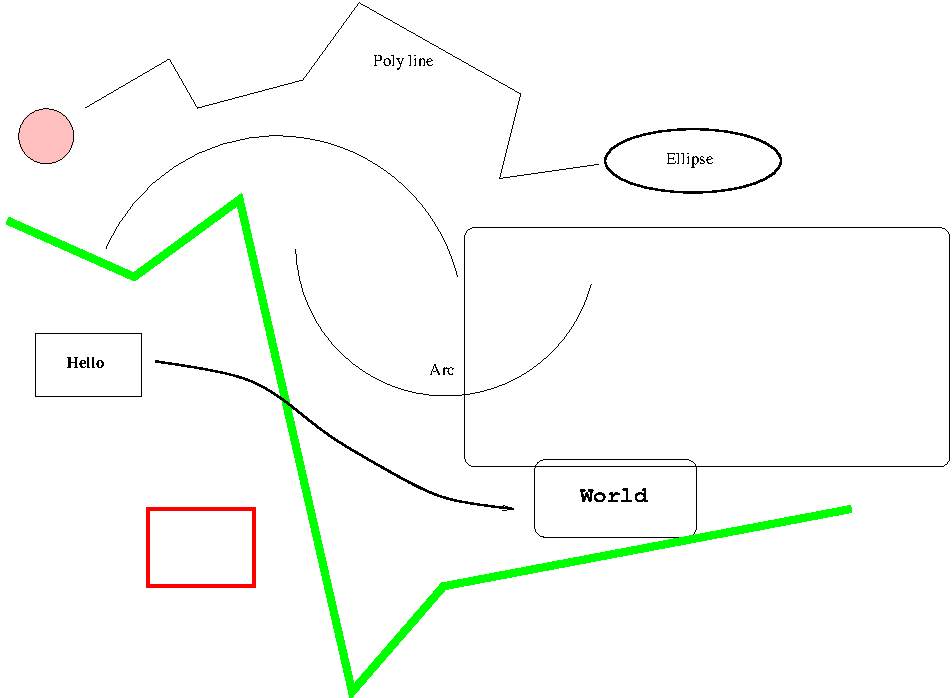
\includegraphics{figs/diagram.pdf}}
\caption{Example diagram drawn using \texttt{xfig}}
\label{xfig}
\end{figure}


\chapter{Evaluation}

\section{Printing and binding}

Use a ``duplex'' laser printer that can print on both sides to print
two copies of your dissertation. Then bind them, for example using the
comb binder in the Computer Laboratory Library.

\section{Further information}

See the Unix Tools notes at

\url{http://www.cl.cam.ac.uk/teaching/current-1/UnixTools/materials.html}


\chapter{Conclusion}

I hope that this rough guide to writing a dissertation is \LaTeX\ has
been helpful and saved you time.


%%%%%%%%%%%%%%%%%%%%%%%%%%%%%%%%%%%%%%%%%%%%%%%%%%%%%%%%%%%%%%%%%%%%%
% the bibliography
\begin{thebibliography}{1}
\addcontentsline{toc}{chapter}{Bibliography}

\bibitem{rust} Rust, a modern low level programming language, https://www.rust-lang.org/
\bibitem{ipv6_rfc} Internet Protocol, Version 6 (IPv6) Specification, RFC 8200, July 2017
\bibitem{mininet} Mininet, a network virtualisation library in Python, http://mininet.org/

\end{thebibliography}

%%%%%%%%%%%%%%%%%%%%%%%%%%%%%%%%%%%%%%%%%%%%%%%%%%%%%%%%%%%%%%%%%%%%%
% the appendices
\appendix

\chapter{Latex source}

\section{diss.tex}
{\scriptsize\verbatiminput{diss.tex}}

\section{proposal.tex}
{\scriptsize\verbatiminput{proposal.tex}}

\chapter{Makefile}

\section{makefile}\label{makefile}
{\scriptsize\verbatiminput{makefile.txt}}

\section{refs.bib}
{\scriptsize\verbatiminput{refs.bib}}


\chapter{Project Proposal}

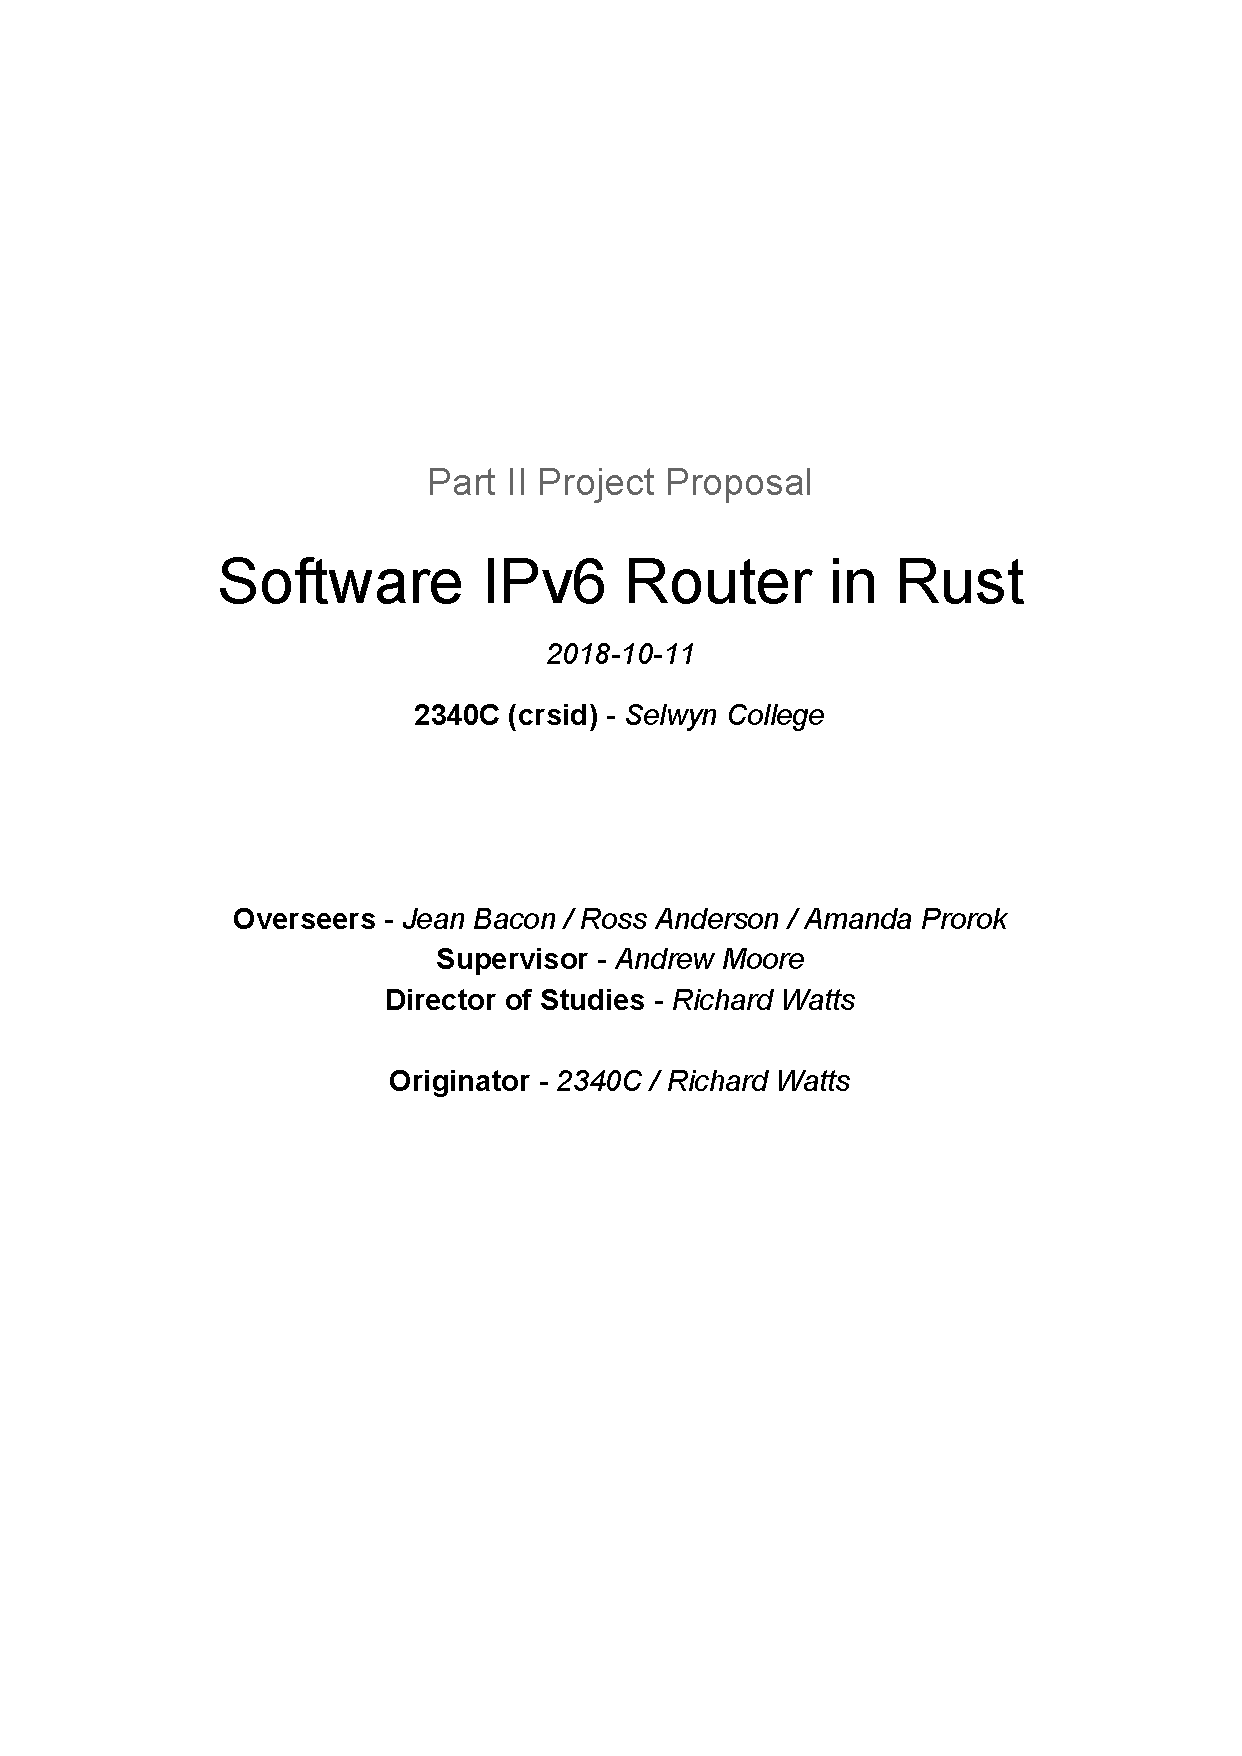
\includepdf[page=-]{proposal}

\end{document}